\section{Data preprocessing}

\subsection{Know your data}

First step: Make sure data is from a reliable provider.

Second step: Look at summary statistics. This includes first order moments (mean, median, etc.), but second order quantities (variance, covariance/correlation) are useful as they can hint at colinearities in data. 

Often models include so many predictors that it is unpractical to look at these metrics. Minimal verification is recommended. 
\begin{itemize}
    \item focus on a subset of predictors (e.g., the most important or ones commonly linked to factors);
    \item track outliers in the summary statistics (when maximum/median or median/minimum ratios are off).
\end{itemize}

Below is an example showing the distribution of correlations between features and the one month ahead return.
\begin{figure}[H]
    \centering
    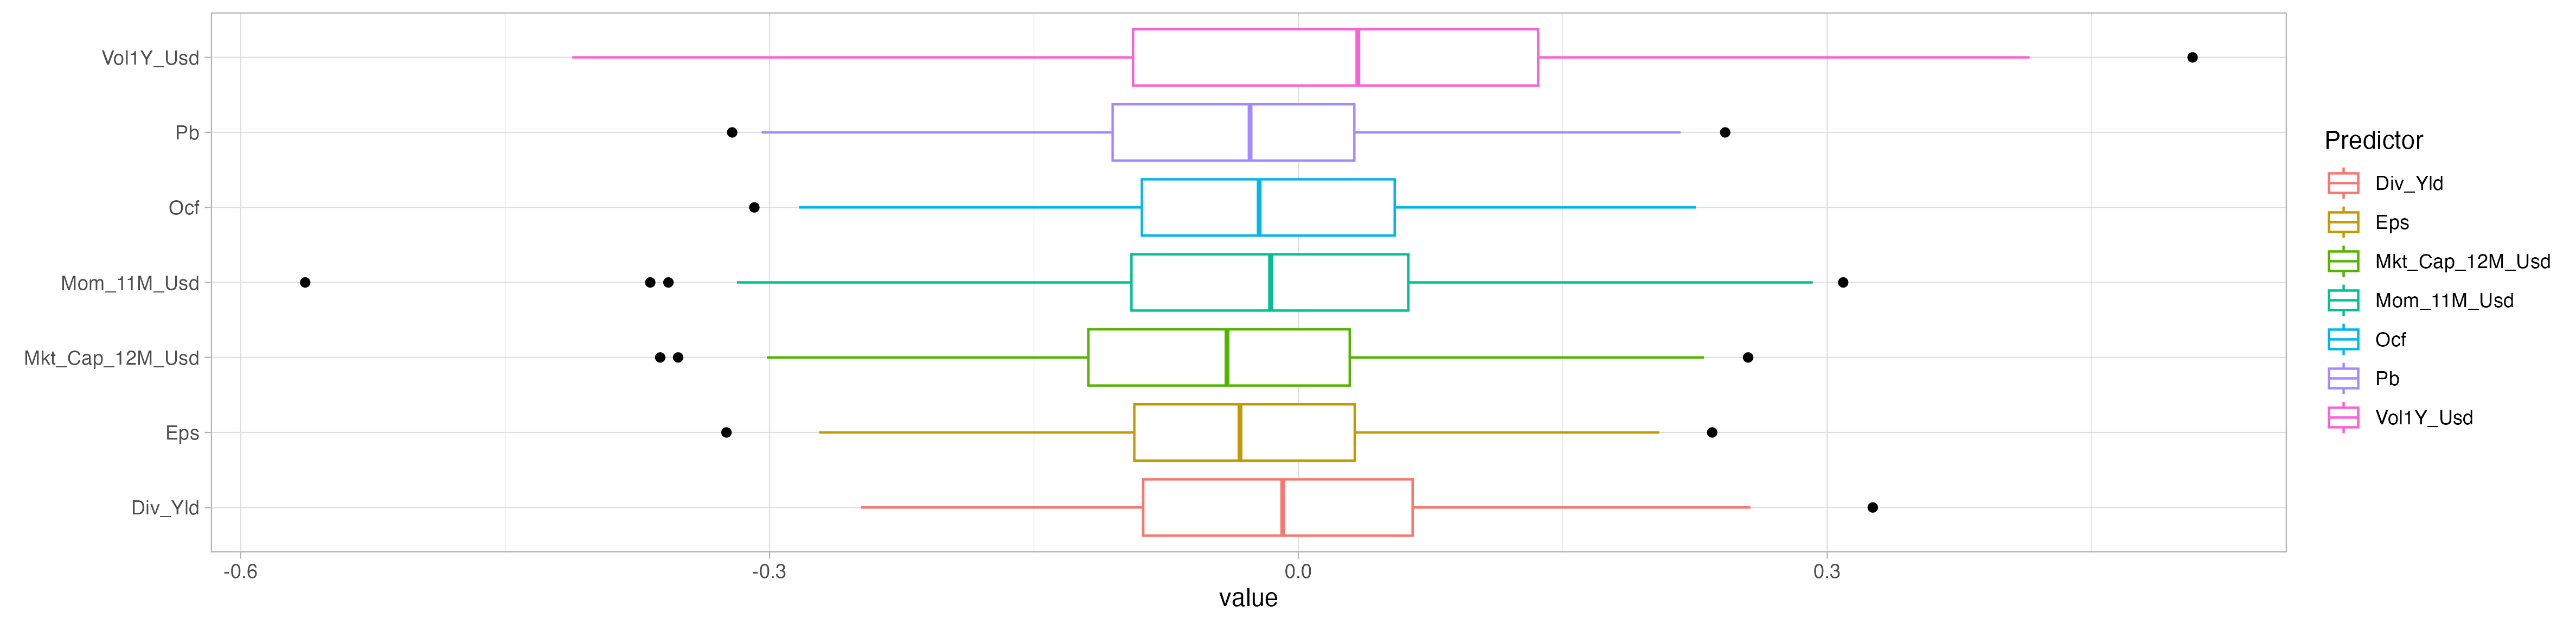
\includegraphics[width=\textwidth]{part_1/images/know_your_data_fig_1:boxplot.png}
\end{figure}

An important metric is the \textbf{smoothed conditional average} of the dependent variable on one feature. This can show the impact of a simple feature. 

Assume only one feature $X$ and we have the model $Y = f(X) + \text{error}$. The function $f$ which minimizes that average squared error $f(x) = \mathbb{E}[ (Y - f(X))^{2}]$ is the regression function:
\begin{equation}
    f(x) = \mathbb{E}[Y | X = x]
\end{equation}

Two examples of such a function are shown below, where the dependent variable is the one month ahead return. Note that both predictors have been uniformized (see later sections), so their values are uniformly distributed in the cross-section of assets for any given time period. The range of features is therefore $[0,1]$. Notice that the confidence interval is narrow when both (i) many data points are available, (ii) these datapoints are not too dispersed.
\begin{figure}[H]
    \centering
    
\includegraphics[width=\textwidth]{part_1/images/know_your_data_fig_2:sca.png}
\end{figure}
The two variables have a close to monotonic impact on future returns. Returns, on average, decrease with market capitalization (thereby corroborating the so-called size effect). The reverse pattern is less pronounced for volatility.


One important empirical property of features is autocorrelation (or absence thereof). A high level of \textbf{autocorrelation} for one predictor makes it plausible to use simple imputation techniques when some data points are missing. But autocorrelation is also important when moving towards prediction tasks. Autocorrelation has been calculated feature-by-feature and stock-by-stock in the plot below 
\begin{figure}[H]
    \centering
    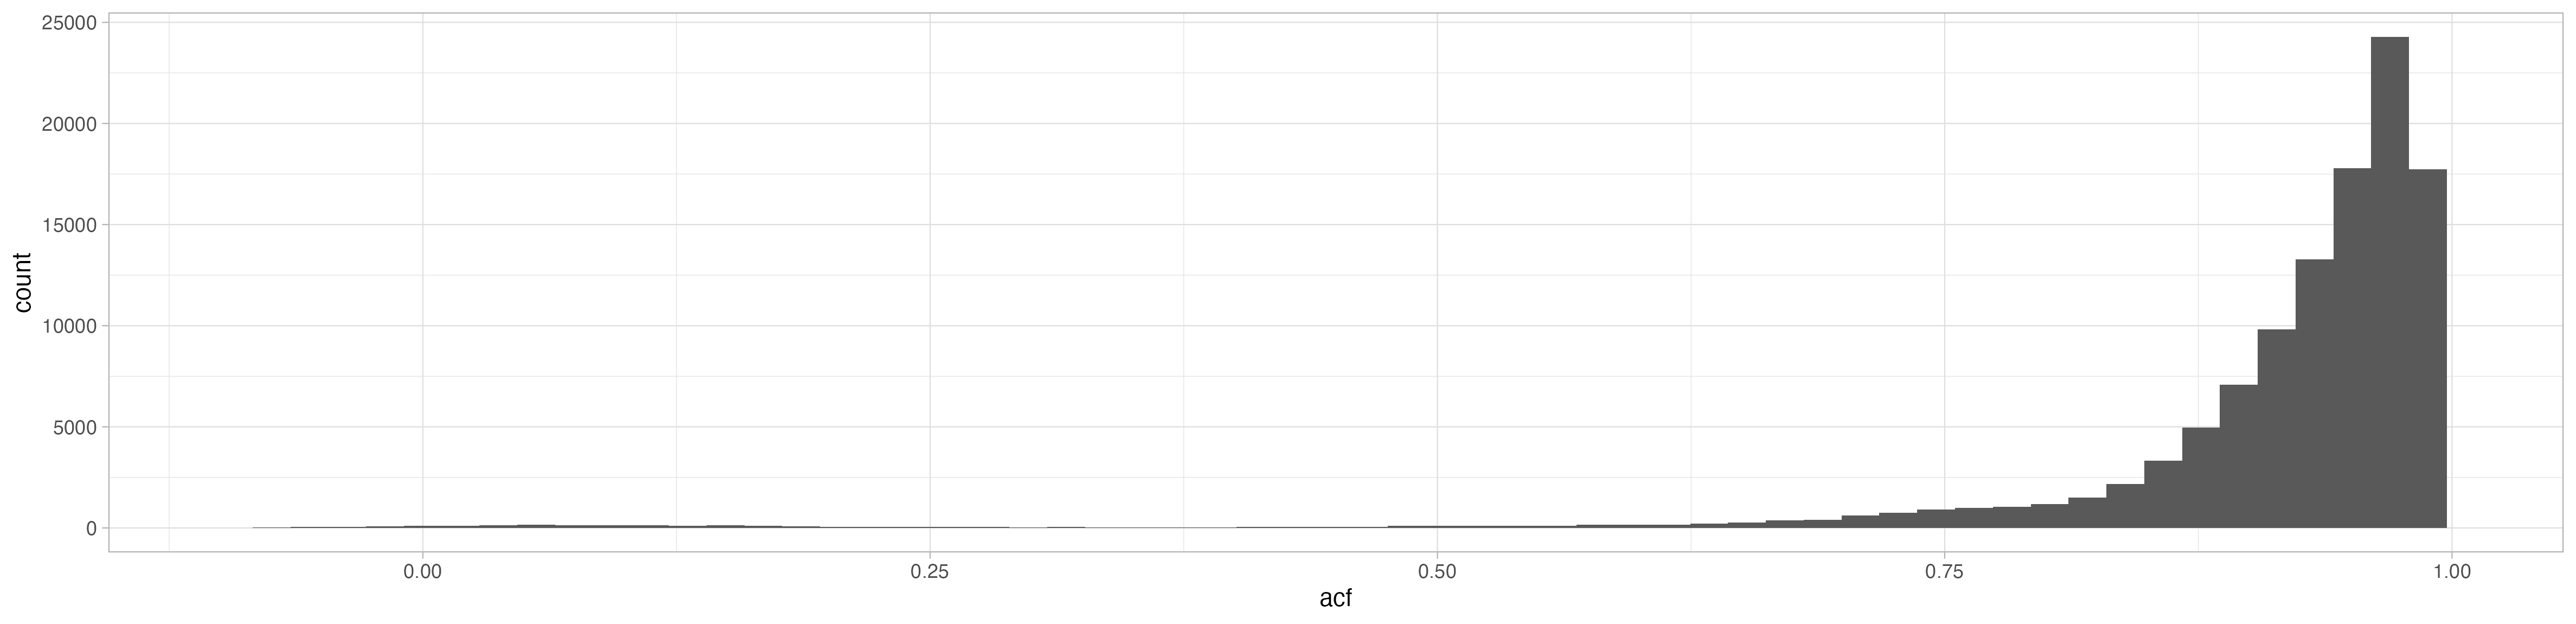
\includegraphics[width=0.6\textwidth]{part_1/images/know_your_data_fig_3:autocorr.png}
\end{figure}


We can see that predictors are highly correlated: most of them have autocorrelation around $0.8$.

\subsection{Missing data}
The methods for handling missing data are plentiful, but a simple heuristic approach is often sufficient. There are two ways of handling missing data: \textbf{removal} and \textbf{imputation}.Removal is agnostic but costly, especially if one whole instance is eliminated because of only one missing feature value. Imputation is often preferred but relies on some underlying and potentially erroneous assumption. 

Below is a simplified classification of imputation:
\begin{itemize}
    \item A basic imputation choice is the median (or mean) of the feature for the stock over the past available values. If there is a trend in the time series, this will nonetheless alter the trend. 
    \item In time series contexts with views towards backtesting, the most simple imputation comes from previous values: if $x_{t}$ is missing replace it with $x_{t-1}$. In some cases this is a very bad choice (see below).
    \item Medians and means can also be computed over the \textbf{cross-section} of assets. This roughly implies that the missing feature value will be relocated in the bulk of observed values. When many values are missing, this creates an atom in the distribution of the feature and alters the original distribution. One advantage is that this imputation is not forward-looking. 
    \item Other techniques rely on modelling assumptions for data generation. This will refer to non parametric approaches, which rely on random forests, Bayesian imputation, maximum likelihood approaches, interpolation or extrapolation adn nearest neighbor algorithms. Advanced techniques are much more demanding computationally.
\end{itemize}

A word of caution: 
\begin{itemize}
    \item Interpolation should be avoided at all costs. For example: Accounting values or ratios that are released every quarter must never be linearly interpolated for the simple reason that this is forward-looking. If numbers are disclosed in January and April, then interpolating February and March requires the knowledge of the April figure, which, in live trading will not be known. Resorting to past values is a better way to go.
    \item There are some feature types where imputation from past values should be avoided. E.g., returns should not be replicated. A better choice is to set the missing returns to zero (which is often close to the median or mean). An indicator that can be used in the decision is autocorrelation, which is the persistence of the feature through time. If a feature is highly autocorrelated then imputation from past values can make sense. If not, then avoid imputation. 
    \item There are cases that require more attention, and there are no out-of-the-box solutions. Consider a case of dividend yield released quarterly, in March, June, September, etc. We know the March value, but in June the data is missing. We do not know if there is a collection error where, or if the firm simply did not pay out any dividend in June. There are no perfect solutions, but for dividend data three options are: 1) Keep the previous value (use \codetext{na.locf()} is very good at this), 2) extrapolate from previous observations, 2) Set to zero (my be suboptimal due to dividend smoothing practices). For persistent time series the first two options are preferred.
\end{itemize}

Tests can be performed to evaluate the relative performance of each option. It is also important to remember these design choices. There are so many of them that they are easy to forget. Keeping track of them is obviously compulsory


\subsection{Outlier detection}
Incredibly sophisticated methods may require a lot of efforts for possibly limited gain. Simple heuristic methods, as long as they are documented in the process, may suffice. They often rely on hard thresholds
\begin{itemize}
    \item For one given feature (possibly filtered in time) any point outside the interval $[\mu - m \cdot \sigma; \mu + m \cdot \sigma]$ where often $m \in \{ 3,5,10 \} $ can be considered an outlier. 
    \item If the largest value is $m$ times above the second-to-largest, then it can be considered an outlier.
    \item For a give small threshold $q$, any value outside the $[q; 1-q]$ quantile range can be considered an outlier. 
\end{itemize}

The last idea is called \textbf{Winsorizing}, which is done by setting all values below $x^{(q)}$ to $x^{(q)}$ and values above $x^{(1-q)}$ to $x^{(1-q)}$. The winsorized variable is $\tilde{x}$
\[
    \tilde{x}_i = \begin{cases}
    x_{i} & \text{if } x_{i} \in [x^{(q)}, x^{(1-q)}] \\
    x^{(q)} & \text{if } x_{i} < x^{(q)} \\
    x^{(1-q)} & \text{if } x_{i} > x^{(1-q)} 
    \end{cases}
\]
where $q$ usually is $(0.5\%, 5\%)$ with 1\% and 2\% being the most commonly used. The winsorization stage \textbf{must} be performed on a feature-by-feature and a date-by-date basis.

We conclude this subsection by recalling that true outliers (i.e., extreme points that are not due to data extraction errors) are valuable because they are likely to carry important information.

\subsection{Feature engineering}
“Garbage in, garbage out”. It is paramount to prevent the ML engine of the allocation to be trained on ill-designed variable.

\subsubsection{Feature selection}
One heuristic choice is to chose the variables that are often mentioned in the literature (both academic and practical). Though of course, sticking to common characteristics may complicate the generation of alpha because all trading agents will take them into account. Choices can stem from empirical studies such as A. Y. Chen and Zimmermann (2021), or theoretical models like Ohlson (1995). 

Then, given a large set of predictors, it seems a sound idea to filter out unwanted or redundant exogenous variables. Heuristically, simple methods include:
\begin{itemize}
    \item computing the correlation matrix of all features and making sure that no (absolute) value is above a threshold (0.7 is a common value) so that redundant variables do not pollute the learning engine;
    \item carrying out a linear regression and removing the non significant variables (e.g., those with $p$-value above $0.05$);
    \item perform a clustering analysis over the set of features and retain only one feature within each cluster.
\end{itemize}

Both these methods are somewhat reductive and overlook nonlinear relationships. Another approach would be to fit a decision tree (or a random forest) and retain only the features that have a high variable importance. 

\subsubsection{Scaling the predictors}
The premise of the need to pre-process the data comes from the large variety of scales in financial data. While it is widely considered that monotonic transformations of the features have a marginal impact on prediction outcomes, Galili and Meilijson (2016) show that this is not always the case. 

If we write $x_{i}$, for the raw input and $\tilde{x}_i$ for the transformed data, common scaling practices include:
\begin{itemize}
    \item \textbf{standardization}: $\tilde{x}_{i} = (x_{i} - m_{x}) / \sigma _{x}$, where $m_{x}$ and $\sigma _{x}$ are the mean and standard deviation of $x_{i}$;
    \item \textbf{min-max} rescaling over $[0,1]$: $\tilde{x}_{i} = (x_{i} - \mathrm{min}(\mathbf{x})) / (\mathrm{max}(\mathbf{x}) - \mathrm{min}(\mathbf{x}))$; 
    \item \textbf{min-max} rescaling over $[-1,1]$: $\tilde{x}_i = 2 \cdot \frac{x_{i} - \mathrm{min}(\mathbf{x})}{\mathrm{max}(\mathbf{x}) - \mathrm{min}(\mathbf{x})} - 1$;
    \item \textbf{uniformization}: $\tilde{x}_i = F_{\mathbf{x}}(x_{i})$ , where $F_{\mathbf{x}}$ is the empirical c.d.f of $\mathbf{x}$. $\tilde{\mathbf{x}}$ is a vector uniformly distributed over $[0,1]$.
\end{itemize}

Sometimes, it is possible to apply a logarithmic transform of variables with both large values (market capitalization) and large outliers. The scaling can come after this transformation.

It is often advised to scale inputs so that they range in $[0,1]$ before sending them through the training of neural networks for instance.

In factor investing, the scaling of features must be \textbf{operated separately for each date and each feature}. This point is critical. It makes sure that for every rebalancing date, the predictors will have a similar shape and do carry information on the cross-section of stocks.

Scaling features across dates should be proscribed. Take for example the case of market capitalization. In the long run (market crashes notwithstanding), this feature increases through time. Thus, scaling across dates would lead to small values at the beginning of the sample and large values at the end of the sample. This would completely alter and dilute the cross-sectional content of the features.

\subsection{Labelling}

\subsubsection{Simple labels}
There are several ways to define labels when constructing portfolio policies. Of course, the finality is the portfolio weight, but it is rarely considered as the best choice for the label

Usual labels in factor investing are the following:
\begin{itemize}
    \item raw asset returns;
    \item future relative returns (versus some benchmark: market-wide index, or sector-based portfolio for instance). One simple choice is to take returns minus a cross-sectional mean or median;
    \item the probability of positive return (or of return above a specified threshold);
    \item the probability of outperforming a benchmark (computed over a given time frame);
    \item the binary version of the above: YES (outperforming) versus NO (underperforming);
    \item risk-adjusted versions of the above: Sharpe ratios, information ratios, MAR or CALMAR ratios.
\end{itemize}

When creating binary variables, it is often tempting to create a test that compares returns to zero. This is suboptimal because it is very time-dependent. It is a better idea to split the returns in two by comparing them to their time-$t$ median (or average). In this case, the indicator is relative and the two classes are much more balanced.



\subsubsection{Categorical labels}
In a typical ML analysis, when $y$ is a proxy for future performance, the ML engine will try to minimize some distance between the predicted value and the realized values. For mathematical convenience, the sum of squared error ($L^{2}$ norm) is used because it has the simplest derivative and makes gradient descent accessible and easy to compute.

Sometimes, it can be interesting not to focus on raw performance proxies, like returns or Sharpe ratios, but on discrete investment decisions, which can be derived from these proxies. A simple example (decision rule) is the following
\begin{equation}
    y_{t,i} = \begin{cases}
    -1 & \text{if } \hat{r}_{t,i} < r_{-} \\
    0 & \text{if } \hat{r}_{t,i} \in [r_{-}, r_{+}] \\
    1 & \text{if } \hat{r}_{t,i} > r_{+}
    \end{cases}
\end{equation}
where $\hat{r}_{t,i}$ is the performance proxy, $r_{\pm}$ are decision thresholds, and $-1$, $0$, and $1$ are the decisions (e.g., sell, hold, buy). It is often recommended that $r_{\pm}$ are chosen so the three categories are relatively balanced (have the same number of observations).

In this case, the final output can be considered as categorical or numerical because it belongs to an important subgroup of categorical variables: the ordered categorical (\textbf{ordinal}) variables. If $y$ is taken as a number, the usual regression tools apply.

When $y$ is treated as a non-ordered (\textbf{nominal}) categorical variable, then a new layer of processing is required because ML tools only work with numbers. Hence, the categories must be recoded into digits. The mapping that is most often used is called \textbf{one-hot encoding}. The vector of classes is split in a sparse matrix in which each column is dedicated to one class. The matrix is filled with zeros and ones. A one is allocated to the column corresponding to the class of the instance.

From the standpoint of allocation, handling categorical predictions is not necessarily easy. For long-short portfolios, plus or minus one signals can provide the sign of the position. For long-only portfolio, two possible solutions: (i) work with binary classes (in versus out of the portfolio) or (ii) adapt weights according to the prediction: zero weight for a -1 prediction, 0.5 weight for a 0 prediction and full weight for a +1 prediction. Weights are then of course normalized so as to comply with the budget constraint.

\subsubsection{Filtering the sample}
One of the main challenges in Machine Learning is to extract as much \textbf{signal} (patterns that will hold out-of-sample) as possible. Intuitively, it may seem reasonable to think that the more data we gather, the more signal we can extract. This is in fact false in all generality because more data also means more noise. Filtering the training samples can improve performance.

In Coqueret and Guida (2020), we investigate why smaller samples may lead to superior out-of-sample accuracy for a particular type of ML algorithm: decision trees (see Chapter 6). We focus on a particular kind of filter: we exclude the labels (e.g., returns) that are not extreme and retain the 20\% values that are the smallest and the 20\% that are the largest (the bulk of the distribution is removed). In doing so, we alter the structure of trees in two ways:
\begin{itemize}
    \item when the splitting points are altered, they are always closer to the center of the distribution of the splitting variable (i.e., the resulting clusters are more balanced and possibly more robust);
    \item the choice of splitting variables is (sometimes) pushed towards the features that have a monotonic impact on the label.
\end{itemize}

These two properties are desirable. The first reduces the risk of fitting to small groups of instances that may be spurious. The second gives more importance to features that appear globally more relevant in explaining the returns. However, the filtering must not be too intense (10\% filtering removes to much signal).

Several horizons come into play during the whole ML-driven allocation workflow: the \textbf{horizon of the label} (time period over which the outcome (label) is observed), the \textbf{estimation window} (chronological depth of the training samples / how much past data is used for training the model) and the \textbf{holding periods}. A paper analyzed different horizons for labels and holding (3,6,9,12). While there is no machine learning whatsoever in this contribution, it is possible that their conclusion that horizons matter may also hold for more sophisticated methods. This topic is in fact much discussed, as is shown by the continuing debate on the impact of horizons in momentum profitability.

This debate should also be considered when working with ML algorithms. In the present chapter, the horizon of the label is the important ingredient. Heuristically, there are four possible combinations if we consider only one feature for simplicity:
\begin{enumerate}
    \item oscillating label and feature;
    \item oscillating label, smooth feature (highly autocorrelated);
    \item smooth label, oscillating feature;
    \item smooth label and feature.
\end{enumerate}

Of all of these options, the last one is probably preferable because it is more robust. 


A pattern that holds between two slowly moving series is more likely to persist in time. Thus, since features are often highly autocorrelated, combining them with smooth labels is probably a good idea.

To illustrate how critical this point is, we will purposefully use 1-month returns in most of the examples of the book and show that the corresponding results are often disappointing. These returns are very weakly autocorrelated while 6-month or 12-month returns are much more persistent and are better choices for labels.

Theoretically, assume that returns are explained entirely by one feature $x_{t}$: $r_{t+1} = f(x_{t}) + \varepsilon_{t}$, where $x_{t}$ is highly autocorrelated and $\varepsilon_{t}$ is small. The compounded interest over multiple periods $(1 + r_{t+1}) (1 + r_{t+2}) - 1$ contains more meaningful signal than just $r_{t+1}$ alone. This suggests that incorporating memory effects into models (e.g., using longer time horizons or recurrent architectures) can improve predictions.

\subsection{Handling persistence}
Feature engineering and labelling have been separated into two different subsections, however i is best to consider them jointly. One important property of the dataset processed by the ML algorithm should be the consistency of persistence between features and labels. This means that autocorrelation patterns between label $y_{t,n}$ and the features $x_{t,n}^{(k)}$ should not be to distant.

Among other more technical options, there are two simple solutions when facing this issue: either introduce autocorrelation into the label, or remove it from the features. Again, the first option is not advised for statistical inference on linear models. Both are rather easy econometrically:
\begin{itemize}
    \item to increase the autocorrelation of the label compute performance over longer time ranges. For instance, when working with monthly data, considering annual or biennial returns will do the trick.
    \item To get rid of autocorrelation, the quickest way to do so is to resort to differences: $\Delta x_{t,n}^{(k)} = x_{t,n}^{(k)} - x_{t-1,n}^{(k)} $. An advantage of this procedure is that it makes sense, economically: variations in features my be better drivers of performance, compared to raw levels.
\end{itemize}

\subsection{Extensions}
\subsubsection{Transforming features}
The feature space can be augmented with simple operations. One of them is lagging (i.e., considering older values of features and assuming some memory effect for their impact on the label). This is useful mostly if the features are oscillating (adding a layer of memory on persistent feature can be redundant). New variables are defined by $\breve{x}_{t,n}^{(k)} = x_{t-1,n}^{(k)}$. 

In some cases (e.g., insufficient number of features), it is possible to consider ratios or products between features. Accounting ratios like price-to-book, book-to-market, debt-to-equity are examples of functions of raw features that make sense. The risk of overfitting increases, just like in a simple linear regression adding variables mechanically increases the $R^{2}$.

Another way to increase the feature space (mentioned above) is to consider differences. In this case, a new predictor is $\breve{x}_{t,n}^{(k)} = x_{t,n}^{(k)}  - x_{t-1,n}^{(k)}$.

\subsubsection{Macro-economic variables}
The data should never be separated from the context it comes from (its environment). In classical financial terms, this means that a particular model is likely to depend on the overarching situation which is often proxied by macro-economic indicators. One way to take this into account at the data level is simply to multiply the feature by an exogenous indicator $z_{t}$ and in this case, the new predictor is $\breve{x}_{t,n}^{(k)} = z_{t} \times x_{t,n}^{(k)}$.

Another route that integrates shifting economic environments is conditional engineering. Suppose that labels are coded via formula (4.2). The thresholds can be made dependent on some exogenous variable. It might be a good idea to adjust the thresholds based on the macro-economic state. One such example of dynamic thresholding is
\begin{equation}
    r_{t, \pm} = r_{\pm} \times e^{\pm \delta (\mathrm{VIX}_t - \bar{\mathrm{VIX}})}
\end{equation}
where $\mathrm{VIX}_{t}$ is the $t$ time value of the VIX index, and $\bar{\mathrm{VIX}}$ is some average og median value. The parameter $\delta $ tunes the magnitude of correction.